% vim: ft=tex
\chapter{Scope}
This technical goals of this bachelor thesis include extending mindclue GmbH's
Roadster framework by adding features such as clustering, high availability and
transport security.

\section{Motivation}
TODO Why do we care about this thesis? Why are we interested?

ruby, \zmq, learning more about zmq, actor model (shared nothing architecture), high availability, real use case, cztop, cztop-patterns, latex, improving english skills, awesome teacher, potential future job position, testimonial/reference, knowledge spreading (of Roadster)

\section{Initial Situation}

\subsection{mindclue GmbH}
\subsubsection{About}
Die Firma mindclue GmbH mit Sitz in Ziegelbrücke GL/SG stellt für ihren
Partner REMTEC AG für Steuerungen, Regelungen und Überwachungen von technischen Prozessen,
komplette SCADA- und Steuerungssysteme her. Dabei sind sie in den Bereichen
Betriebs-und Sicherheitausrüstung für Nationalstrassen, Trinkwasser-
versorgungen, im Energiesektor und vielen Spezielbereichen tätig.
Dabei setzen sie auf ihre eigens entwickelte Applikation - Roadster.

\subsubsection{Roadster}
Roadster ist eine Ereignis gesteuerte Applikation geschrieben in Ruby.
Sie ist die eigentliche SCADA Applikation und wird bereits in einer Vielzahl von
Tunnelanlagen in der Schweiz eingesetzt und dient zur Überwachung der einzelnen Komponenten im Tunnel.
Durch den modularen Aufbau kann jede Roadster Applikation sich selbst laufen - Autonom.
Sprich jeder Roadster hat seinen eigenen Webserver und Datenverwaltung.

\subsubsection{AS - UeLS}
Roadster ist einer von vielen AS Knoten eines UeLS. Die Kommunikation
zwischen AS und AR geschieht über "OPC UA".
%TODO .... include graphics as_detail and overall system


\subsection{\zmq}
\emph{For a more detailed introduction, see \autoref{ch:zmq}.}
%TODO add acronyms/abbreviations to glossary (TIPC, TCP, PGM, MOM, BSD, NaCl, ...)
To understand Roadster's architecture and the rest of this document, it's
helpful to understand the basics of \zmq (sometimes written as ZeroMQ or simply
ZMQ) first. This is a brief introduction to \zmq for the unfamiliar reader.

\zmq is a MOM implemented as an open source library, that is, it doesn't
require a dedicated broker. Instead, it offers sockets with an abstract
interface similar to BSD sockets. Different types of sockets are used for
different messaging patterns such as request-reply, publish-subscribe, and
push-pull.

A single socket can bind/connect to multiple endpoints, which allows \zmq to
use round-robbin on the sender side, and fair-queueing on the receiver side,
where applicable. It doesn't matter whether the communication happens
in-process (between threads), inter-process (e.g. over Unix Domain Sockets), or
inter-node (e.g. over TCP/PGM/TIPC), since the transport is completely
abstracted away. The same goes for connection handling; an arbitrary amount of
connections is handled over a single socket and reconnecting after short
network failures is done transparently.

\zmq is lightweight and provides extremely low latencies, which means it can
also be used as the fabric of concurrent applications, e.g. for the actor
model. In case of the TCP transport, it incorporates advanced techniques such
as smart message batching to achieve significantly higher throughputs than with
raw TCP or other MOM solutions \cite[Figure 2, Middleware evaluation and
prototyping, p.~4]{cern:new-cmw}.

To build a solution with \zmq, its sockets are used as building blocks to
design custom message flows. Certain patterns are used to achieve reliability
with respect to the failure types that need to be addressed in particular.  The
zguide\footnote{\url{http://zguide.zeromq.org/}} explains best practices,
including commonly needed, resilient messaging patterns.

The above characteristics make \zmq a valuable asset when it comes to building
robust, distributed high-performance systems.

\subsubsection{Transport Security}
Since version 4.0, \zmq boasts state of the art encryption and authentication,
based on the excellent and highly renown
NaCl\footnote{\url{http://nacl.cr.yp.to}} library.

\subsubsection{Data Serialization}
Data serialization is outside the scope of \zmq. To fill the gap, one typically
uses another library such as MsgPack\footnote{\url{http://msgpack.org}},
Protocol
Buffers\footnote{\url{https://developers.google.com/protocol-buffers/}}, or
even a programming language's built-in object serialization
support\footnote{such as Ruby's marshalling support:
\url{http://ruby-doc.org/core/Marshal.html}}.

\subsubsection{CZMQ}
CZMQ is a high-level abstraction layer for \zmq. It makes working with the \zmq
library more expressive and allows for better portability. It also provides
additional functionality such as a reactor, a simple actor implementation, as
well as utilities for certificate and authentication handling, and LAN node
discovery. This is the recommended way of using \zmq nowadays.

\subsection{Software Architecture}
TODO Roadster architecture\\

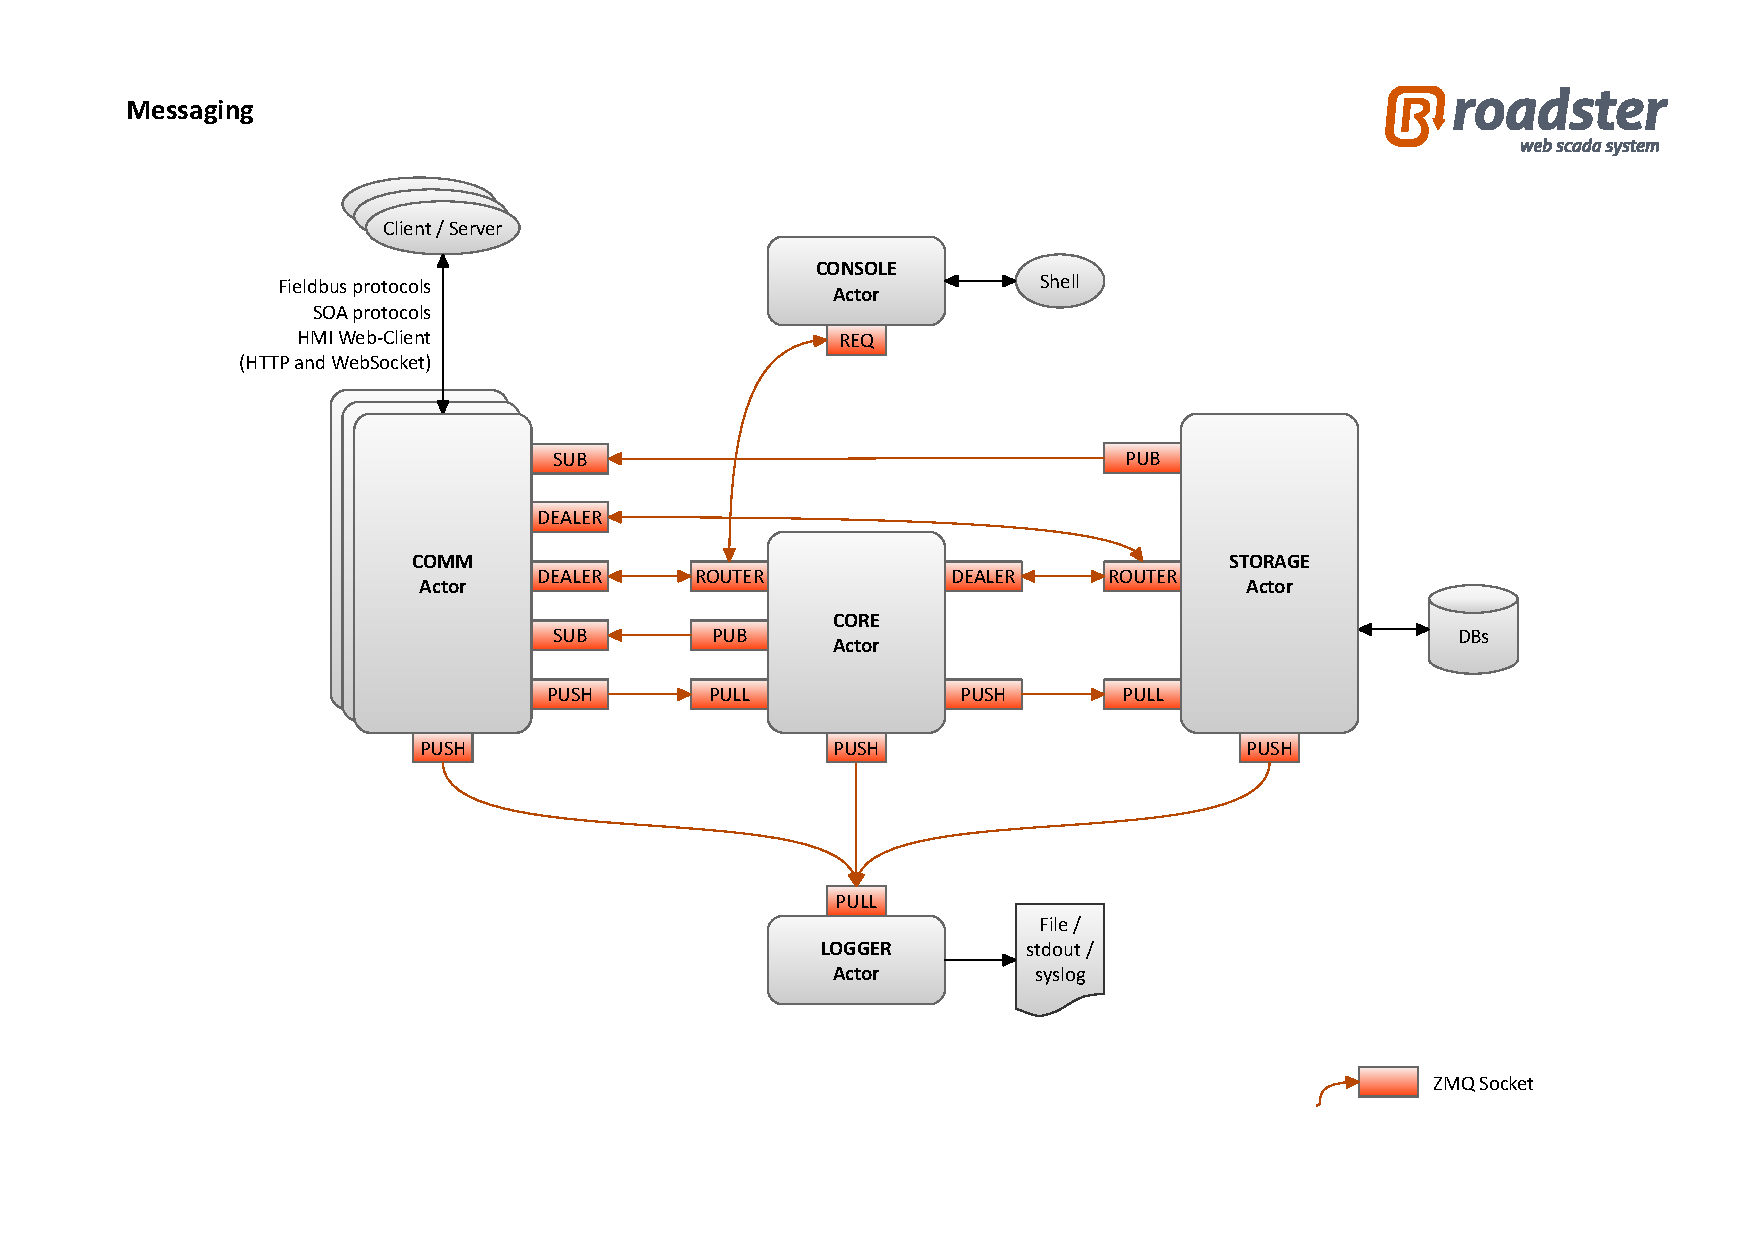
\includegraphics[trim=4cm 2cm 3.5cm 2.8cm, clip=true, width=\textwidth]{img/roadster_arch.pdf}

\section{Goals}
TODO mandatory goals

\subsection*{Optional Goals}
TODO optional goals
